\documentclass[final]{article}

\PassOptionsToPackage{numbers,compress}{natbib}
\usepackage{APS360}
\usepackage{amsmath}
\usepackage[utf8]{inputenc} % allow utf-8 input
\usepackage[T1]{fontenc}    % use 8-bit T1 fonts
\usepackage{hyperref}       % hyperlinks
\usepackage{url}            % simple URL typesetting
\usepackage{booktabs}       % professional-quality tables
\usepackage{amsfonts}       % blackboard math symbols
\usepackage{nicefrac}       % compact symbols for 1/2, etc.
\usepackage{microtype}      % microtypography
\usepackage{xcolor}         % colors
\usepackage{graphicx}       % include graphics
\DeclareMathOperator{\sinc}{sinc}
\begin{document}
\vspace{-20pt}

\href{https://github.com/noshou/APS360/tree/main}{\textbf{Github Repo}}



%==============================================================================
\section{Introduction and Background}
%==============================================================================

X-ray scattering produces a 1-D intensity profile $I(q)$ that encodes the 3-D shape of a
molecule, but computing it exactly via the Debye equation scales as $O(N^2)$ in atom count,
making it prohibitively slow for large structures and incompatible with gradient-based
optimization. This proposal seeks to answer the question 
\emph{can a graph neural network learn to predict $I(q)$ directly from
atomic coordinates?} To answer this, this project aims to train a message-passing GNN as a fast, 
differentiable surrogate for the exact computation. 

Graph neural networks for molecular property prediction were pioneered by
SchNet~\cite{schutt_schnet_2018}, which introduced continuous-filter convolutions on
interatomic distances and remains a strong baseline for scalar molecular properties.
DimeNet~\cite{gasteiger_dimenet_2020} extended this by incorporating bond angles, improving
accuracy on quantum-chemical targets such as the QM9 benchmark~\cite{ramakrishnan_qm9_2014}.
On the scattering side, CRYSOL~\cite{svergun_crysol_1995} established the spherical-harmonic
decomposition approach that we use to generate ground-truth $I(q)$ labels.
More recently, \citet{Schutt2021} introduced PaiNN, an equivariant message-passing network.


When a beam of X-rays is fired at a molecule, each atom deflects (``scatters'') the beam by an
amount that depends on the atom's identity and the deflection angle~$q$. Each atom has a
characteristic \emph{atomic form factor} $f_k(q)$ encoding how strongly it scatters at
angle~$q$. By measuring the total scattered intensity across all angles, we obtain a
\emph{scattering profile} $I(q)$ which is a unique fingerprint of the molecule's 3-D shape~\cite{debye}. The exact formula, 
the \textbf{Debye equation}, sums the pairwise interatomic interactions:
\begin{equation}
    I(q) = \sum_{\alpha}\sum_{\beta}
    f_{\alpha}(q)\,f^{*}_{\beta}(q)\;\sinc\!\bigl(q\,|\mathbf{r}_{\alpha} - \mathbf{r}_{\beta}|\bigr)
    \label{eq:debye}
\end{equation}
where $\sinc(x)=\sin(x)/x$ captures the intuition that atoms far apart interfere less strongly. Because every pair must be evaluated, 
this scales as $O(N^2)$ in the number of atoms. The Stuhrmann decomposition (Eq.~\ref{eq:stuhrmann}) expands the Debye equation into a sum of spherical harmonics, decomposing the
molecular shape into a sum of \(L^2\) angular modes, truncated at order~$L$. This reduces the time complexity down to $O(N \cdot L^2)$, 
and assuming for most cases \(L \ll N\), reduces to $O(N)$~\cite{Stuhrmann}.
This project uses the in-vacuo form (no solvent, hydration shell, or intermolecular forces); a \href{https://noshou.github.io/APS360/}{live demo} is available online.
\begin{equation}
    B_{lm}(q) = \sum_i f_i(q)\,j_l(qr_i)\,Y^*_{lm}(\theta_i,\phi_i),
    \qquad
    I(q) = (4\pi)^2 \sum_{l,m} |B_{lm}(q)|^2
    \label{eq:stuhrmann}
\end{equation}


\section{Data Processing}

A dataset of \textbf{1,139,747 molecules} was assembled from 13 sources with diverse composition.
In total, 474 unique atom/ion types are represented (charge-resolved, e.g.\ \texttt{O} and
\texttt{O2-} are distinct). Full source attributions are provided in \texttt{sources.tsv},
embedded in the database. 
Raw structures were obtained in various formats (.cif, .pdb, .xyz\@) and converted to a
uniform Cartesian XYZ representation. Dummy and non-physical atom sites were removed,
deuterium was mapped to hydrogen, and structures declaring zero atoms were discarded.
Non-element placeholders (\texttt{X}, \texttt{M}, \texttt{Cn}, etc.) were excluded from
the ionic makeup. $I(q)$ ground truths were then computed via the Stuhrmann decomposition 
(\href{https://github.com/noshou/APS360/tree/main/Scattering}{source code})
at $L{=}50$  and stored in a compressed HDF5 database.


%==============================================================================
\section{Proposed Architecture}
%==============================================================================

\begin{figure}[h]
    \centering
    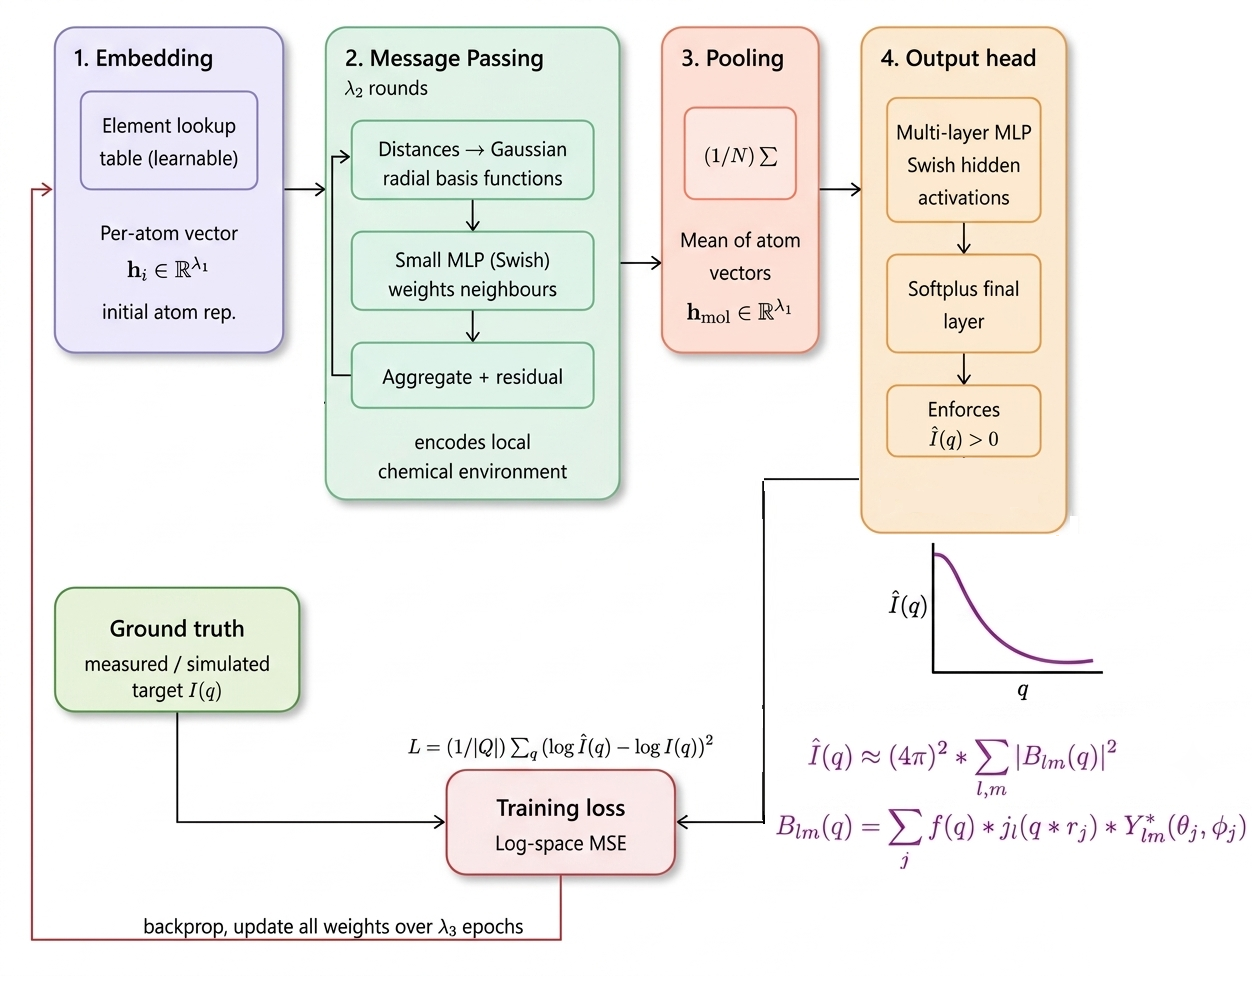
\includegraphics[width=0.8\linewidth]{Gemini_Generated_Image_8yet8b8yet8b8yet.png}
\end{figure}

The proposed network takes a molecule's atomic positions and element types as input and
predicts $\hat{I}(q) \in \mathbb{R}^{|Q|}$. Let hyperparameters $\lambda_1$ be the hidden dimension, $\lambda_2$ the number of 
message-passing rounds, and $\lambda_3$ be the number of training epochs. \textbf{1) Embedding:} 
Atomic coordinate files are converted into a list of atoms, which are looked up in a trainable table, producing a 
vector $\mathbf{h}_i \in \mathbb{R}^{\lambda_1}$. This gives the network a
learnable representation of each element. \textbf{2) Message passing ($\lambda_2$ rounds):} Each atom updates its vector by
aggregating information from nearby neighbours. Interatomic distances are encoded as
Gaussian radial basis functions before being passed to a small MLP (with Swish activations)
that weights each neighbour's contribution. A residual connection is added at each round.
After $\lambda_2$ rounds, each atom's vector encodes its local chemical environment.
\textbf{3) Pooling:} Atom vectors are averaged into a single fixed-size molecule
vector $\mathbf{h}_{\mathrm{mol}} \in \mathbb{R}^{\lambda_1}$, independent of molecule size.
\textbf{4) Output head:} A multi-layer MLP with Swish hidden activations maps
$\mathbf{h}_{\mathrm{mol}}$ to $\hat{I}(q) \in \mathbb{R}^{|Q|}$. A Softplus activation
on the final layer enforces strict positivity $\hat{I}(q) > 0$, consistent with the
physical requirement that scattering intensity is always positive. 
\textbf{5) Backprop:} The model is trained a total of \(\lambda_3\) epochs against ground truths.
The network is trained to minimise a log-scale MSE loss,
\(\mathcal{L} = \frac{1}{|Q|}\sum_{q}\bigl(\log\hat{I}(q) - \log I(q)\bigr)^2\)
which accounts for the orders-of-magnitude variation in intensity across the dataset.


%==============================================================================
\section{Baseline Model}
%==============================================================================

The baseline is a small MLP that takes as input only the atom-type histogram of a molecule
(i.e.\ a count vector $\mathbf{c} \in \mathbb{Z}^{|\mathcal{E}|}$ recording how many atoms of
each element type are present) and maps it directly to $\hat{I}(q) \in \mathbb{R}^{|Q|}$
via two hidden layers with Swish activations and a Softplus output. The model sees no atomic
coordinates, no interatomic distances, and no graph structure whatsoever.

%==============================================================================
\section{Ethical Considerations}
%==============================================================================

All training data is open-source and fully attributed; no private or sensitive information
is involved. The primary risk is misuse of model predictions: since the GNN is an
approximation, predicted $I(q)$ curves could mislead structural biology or materials
research if treated as exact without cross-validation against the ground-truth computation.

\newpage
\bibliographystyle{unsrtnat}
\bibliography{ref}
\end{document}
